\documentclass[11pt]{amsart}
\usepackage[margin=1.1in]{geometry}
\usepackage{amsmath,amssymb,amsthm,mathtools,booktabs,graphicx,hyperref}

\newtheorem{theorem}{Theorem}[section]
\newtheorem{proposition}[theorem]{Proposition}
\newtheorem{lemma}[theorem]{Lemma}
\newtheorem{corollary}[theorem]{Corollary}
\newtheorem{conjecture}[theorem]{Conjecture}
\newtheorem*{theoremA}{Theorem A}
\newtheorem*{theoremB}{Theorem B}
\newtheorem*{theoremC}{Theorem C}
\newtheorem*{theoremD}{Theorem D}
\theoremstyle{definition}
\newtheorem{definition}[theorem]{Definition}
\newtheorem{remark}[theorem]{Remark}
\newtheorem{question}[theorem]{Question}

\newcommand{\F}{\mathbb{F}}
\newcommand{\Z}{\mathbb{Z}}
\newcommand{\N}{\mathbb{N}}
\newcommand{\gr}{\operatorname{gr}}
\newcommand{\rk}{\operatorname{rk}}
\newcommand{\coker}{\operatorname{coker}}
\newcommand{\ad}{\operatorname{ad}}
\newcommand{\hatn}{\widehat{\mathfrak n}}
\newcommand{\Hcal}{\mathcal H}

\title[Mod-2 cokernel density on a non-analytic pro-2 tower]{The mod-2 cokernel density of a Hecke operator on a non-analytic pro-2 tower:\\ split form, explicit kernels, and bounds}
\author{Ruqing Chen}
\address{GUT Geoservice Inc., Montreal, Qu\'ebec, Canada}
\email{ruqing@hotmail.com}
\date{October 2026. DOI: \href{https://doi.org/10.5281/zenodo.23125494}{10.5281/zenodo.23125494}.
Code and data: \url{https://github.com/Ruqing1963/anccft-ce-density}}

\begin{document}

\begin{abstract}
Let $P=(1+\varphi\mathcal O)/(1+t\F_2[[t]])$ be the pro-2 group attached by R.~Chen to the
Cartwright--Mantero--Steger--Zappa $\tilde A_2$-lattice of order $q=2$, where $\mathcal O=\F_8[[\varphi;\sigma]]$,
$\varphi^3=t$, and let $F\in\F_2[\Gamma^0]$ be the element whose right-multiplication cokernel computes the
$\F_2$-corank of the Hecke Laplacian along the canonical tower. Chen asked whether the cokernel density
$c_e$ vanishes, and whether the restricted enveloping algebra of $\gr P$ is a domain.
We answer the second question negatively, exhibiting an explicit square-zero element in degree $4$.
We show that $\gr P\otimes\F_8$ is the positive part of the affine Lie algebra $A_2^{(1)}$ in its principal grading,
so that $\gr P$ is a twisted $\F_2$-form of it, and that the leading form of $F$ is homogeneous of weight
equal to the null root~$\delta$. This yields explicit kernel elements for every level (governed by a ``binary
odometer'' along the imaginary root chain $3\cdot 2^r$), monotonicity statements, and, by exact computation up to
$|G_{10}|=2^{24}$, the bound $c_e\le 0.030322$ (previously $0.0645$). Using evaluation representations of the loop
algebra we prove that the leading form of $F$ is a non-zero-divisor in $\gr\F_2[[P]]$, hence that $F$ is a
non-zero-divisor in $\F_2[[P]]$. Finally we prove that $c_e=0$ follows from two
explicit hypotheses on the kernel of the leading form (verified for $m\le10$ and $m\le14$ respectively), we prove that the
natural level-by-level route to these hypotheses cannot succeed, and we give computational evidence that the zero divisors of
$\gr\F_2[[P]]$ do not lift to $\F_2[[P]]$, consistent with Jaikin-Zapirain's pro-$p$ Atiyah conjecture.
In a last section we treat the analogous graded algebras for all cyclic algebras of degree $\ell$ over $\F_p((t))$:
the non-zero-divisor theorem holds whenever $p\nmid\ell$, the explicit kernels exist only for $(p,\ell)=(2,3)$ (because
of a factor $2$ in a characteristic-$0$ obstruction) and for $\ell=2$, and for $\ell=2$ we find a second explicit kernel
family, coming from the substitution $t\mapsto t^2$, and evidence that the excess over the maximal-rank baseline vanishes.
\end{abstract}

\maketitle

\tableofcontents

%======================================================================
\section{Introduction}
%======================================================================

\subsection{The question}
Let $\F_8=\F_2(\alpha)$ with $\alpha^3=\alpha+1$, $\sigma(a)=a^2$, and let $D$ be the cyclic division algebra
$(\F_8(t)/\F_2(t),\sigma,t)$, i.e.\ $D=\bigoplus_{j<3}\F_8(t)\varphi^j$ with $\varphi a=\sigma(a)\varphi$ and
$\varphi^3=t$. Chen \cite[Thm.~6.4.1]{ChenIII} shows that $a_x\mapsto 1+\alpha^x\varphi$ ($x\in\Z/7$) embeds the
Cartwright--Mantero--Steger--Zappa triangle group $\Gamma$ of order $q=2$ \cite{CMSZ} into $D^\times/\F_2(t)^\times$,
so that $\Gamma$ is a lattice in $PGL_3(\F_2((s)))$, $s=1+t$. Completing at $t=0$, with maximal order
$\mathcal O=\F_8[[\varphi;\sigma]]$, one obtains the pro-2 group
\[
  P=(1+\varphi\mathcal O)/(1+t\F_2[[t]]),\qquad P_m=\operatorname{im}(1+\varphi^m\mathcal O),\qquad G_m=P/P_m ,
\]
with $|G_m|=2^{N_m}$, $N_m=3(m-1)-\lfloor (m-1)/3\rfloor$. The type-preserving subgroup $\Gamma^0$ is dense in $P$;
$P$ is torsion-free, $d(P)=3$, of infinite rank and not $p$-adic analytic \cite[Thm.~6.4.2]{ChenIII}.

With Schreier generators $\theta_{s,x}$ and $\bar f_s=\sum_{x\in\Z/7}\theta_{s,x}^{-1}\in\F_2[G_m]$ put
\[
  F=1+\bar f_1\bar f_0\bar f_2,\qquad C_m=\F_2[G_m]/\F_2[G_m]F,\qquad n_m=3|G_m| .
\]
Then $\dim C_m-1$ is the number of even invariant factors of the Hecke Laplacian of the level-$m$ quotient
complex \cite[Prop.~6.8.3]{ChenIII}, $\dim C_m/n_m$ is non-increasing, and
\[
  c_e:=\lim_{m\to\infty}\dim C_m/n_m
\]
controls the linear growth of the $2$-part of the Hecke Jacobian: $\liminf v_2|\mathrm{Jac}^H(Y_m)|/n_m\ge c_e$
\cite[Thm.~6.8.8]{ChenIII}. Chen asks whether $c_e=0$, and (Remark~6.9.2 of \cite{ChenIII}) whether the
restricted enveloping algebra of $\gr P$ is a domain, which would make $\F_2[[P]]$ a domain.

\subsection{Relation to the pro-$p$ Atiyah conjecture}
By Jaikin-Zapirain \cite[Prop.~11.2]{JZsurvey}, for any pro-$p$ group $G$ and any chain of open normal
subgroups with trivial intersection, $\rk_G(x)=\lim\rk_{\F_p}(x\text{ on }\F_p[G/U_i])/|G:U_i|$ exists and does not
depend on the chain. Hence
\[
  c_e=\tfrac13\bigl(1-\rk_P(F)\bigr)
\]
is intrinsic to $(P,F)$. The pro-$p$ Atiyah conjecture \cite[Conj.~11.1]{JZsurvey} for the torsion-free group $P$
would give $\rk_P(F)=1$, i.e.\ $c_e=0$. It is known for residually torsion-free $p$-adic analytic groups, free
pro-$p$ groups and virtually free-by-$\Z_p$ groups \cite{JZS}, none of which covers $P$. Note that the reduced norm
maps the central subgroup $1+t\F_2[[t]]$ onto itself bijectively (it is cubing on a pro-$2$ group), so that
$P\cong SL_1^1(\widehat D)$, the first principal congruence subgroup of the norm-one group of
$\widehat D=D\otimes_{\F_2(t)}\F_2((t))$;
$P$ is thus an anisotropic analytic group over the local field $\F_2((t))$, a class for which the pro-$p$ Atiyah
conjecture is open. For the analogous questions on the growth of mod-$p$ homology along towers see \cite{EL,Fraczyk}.

\subsection{Main results}
Write $L=\gr P=\bigoplus_{k\ge1}L_k$ for the graded restricted Lie algebra of the filtration $(P_k)$,
$u(L)$ for its restricted enveloping algebra and $u_m=u(L/L_{\ge m})\cong\gr\F_2[G_m]$ (Jennings--Quillen).
Let $\sigma F\in u(L)_3$ be the leading form of $F$.

\begin{theoremA}[Section~\ref{sec:zd}]
$u(L)$ is not a domain. There is a $3$-dimensional subspace $V\subset u(L)_4$ with $V\cdot V=0$; in particular every
$0\ne v\in V$ satisfies $v^2=0$. There are no homogeneous zero-divisor pairs of total degree $\le 7$.
Hence the answer to Remark~6.9.2 of \cite{ChenIII} is negative.
\end{theoremA}

\begin{theoremB}[Section~\ref{sec:split}]
$L\otimes_{\F_2}\F_8$ is isomorphic, as a graded restricted Lie algebra, to the positive part $\hatn$ of the affine
Lie algebra of type $A_2^{(1)}$ in its principal grading, with $2$-map given by matrix squaring. $L$ is the $\F_2$-form
of $\hatn$ twisted by Frobenius composed with the rotation of the affine Dynkin diagram. Under this isomorphism the
leading form $\sigma F$ becomes
\[
  \sigma'=e_0e_1e_2+e_2[e_0,e_1]+e_0[e_1,e_2]+h,\qquad h\in\hatn_\delta ,
\]
which is homogeneous of weight $\delta=\alpha_0+\alpha_1+\alpha_2$ for the affine root grading.
\end{theoremB}

\begin{theoremC}[Sections~\ref{sec:kernel}--\ref{sec:filtration}]
For every $m\ge2$ there are three explicit monomials $\omega_0,\omega_1,\omega_2\in u_m\otimes\F_8\cong u^s_m\otimes\F_8$ of degree
\[
  d(m)=\sum_{k\in\Hcal_m}k,\qquad \Hcal_m=\{1\le k<m:\ 3\nmid k\}\cup\{3\cdot 2^r<m\},
\]
such that $u^s_m\omega_0+u^s_m\omega_1+u^s_m\omega_2$ lies in the kernel of right multiplication by $\sigma F$.
Moreover the first non-injective degree $k_m$ of $R_{\sigma F}$ is non-decreasing in $m$, the kernel density
$\dim\ker R_{\sigma F}/|G_m|$ is non-increasing in $m$, and $k_m\le d(m)\sim m^2/3$.
\end{theoremC}

\begin{theoremD}[Section~\ref{sec:numerics}; exact computation]
$\dim C_7=10226$, and the graded cokernel of $R_{\sigma F}$ on $u_m$ has dimension $64216$, $423412$, $1526176$
for $m=8,9,10$. Consequently
\[
  c_e\le \frac{1526176}{3\cdot 2^{24}}=0.030322\ldots
\]
\end{theoremD}

In Section~\ref{sec:nzd} we prove that right and left multiplication by the leading form are injective on the full
algebra $u(\hatn)$ (Theorem~\ref{thm:nzd}); thus $F$ is a non-zero-divisor in $\F_2[[P]]$ and $k_m\ge m-3$.
In Section~\ref{sec:excess} we split the kernel density as a maximal-rank baseline, which we show is
$O(m^{-1/2})$ (numerically $\approx2.55\,m^{-3/2}$), plus an excess $e_m$ of order $10^{-3}$, and formulate
$c_e=0$ as a Lefschetz-type statement (Conjecture~\ref{conj:excess}). We prove that $c_e=0$ follows from a growth bound
on the kernel below the middle degree together with $k_m\ge d(m)-1$ (Theorem~\ref{thm:conditional}); both hypotheses hold
for $m\le10$, and we show that the excess of $\sigma'$ is a special-position effect: a generic element of the same
weight has maximal rank on every block for $m\le8$. In Section~\ref{sec:lift} we show by exhaustive
linear algebra that every zero-divisor pair of Theorem~A is obstructed at the first or second lifting step in
$\F_2[[P]]$; thus they are artefacts of the filtration and give no counterexample to the pro-2 Kaplansky conjecture.
In Section~\ref{sec:family} we compare with the other cyclic algebras: Theorem~\ref{thm:famnzd} extends the
non-zero-divisor theorem to all $p\nmid\ell$, Proposition~\ref{prop:famcol} shows that the column mechanism behind
Theorem~C is special to $(2,3)$ and $\ell=2$, and Theorem~\ref{thm:famtwo} gives two explicit kernel families for
$\ell=2$, which together with occasional cancellation-type defects account for all computed thresholds there.

\subsection*{Status of the statements}
Results labelled \emph{Theorem}, \emph{Proposition} or \emph{Lemma} have complete proofs here, possibly relying on a
finite exact computation which is then named explicitly (``proof by computation''). All computations are exact
linear algebra over $\F_2$ (over $\F_p$ in Section~\ref{sec:family}) and were cross-checked by independent implementations; see Appendix~\ref{app:comp}.

%======================================================================
\section{The graded algebra}\label{sec:graded}
%======================================================================

\subsection{The Lie algebra $L$}
Let $A=\F_8[\varphi;\sigma]$ (graded by $\deg\varphi=1$); its centre is $\F_2[t]$, $t=\varphi^3$.

\begin{lemma}\label{lem:L}
The filtration $(P_k)$ is a restricted $N$-series and
\[
  L\cong A_{>0}/T,\qquad T=t\F_2[t],
\]
as graded restricted Lie algebras, where $A_{>0}$ carries the commutator bracket and the squaring map. Explicitly,
$L_k=\F_8\varphi^k$ for $3\nmid k$ and $L_k=\F_8\varphi^k/\F_2t^{k/3}$ for $3\mid k$, and
\[
  [a\varphi^i,b\varphi^j]=(a\sigma^i(b)+b\sigma^j(a))\varphi^{i+j},\qquad (a\varphi^k)^{[2]}=a\sigma^k(a)\varphi^{2k}.
\]
\end{lemma}

\begin{proof}
For $x=1+a\varphi^i+\dots$, $y=1+b\varphi^j+\dots$ one has $[x,y]\equiv 1+(a\sigma^i(b)+b\sigma^j(a))\varphi^{i+j}$ and
$x^2\equiv 1+a\sigma^i(a)\varphi^{2i}$ modulo higher order; these are the commutator and square in $A$. The centre
$T$ is closed under squaring, hence a restricted ideal, and quotienting by $1+t\F_2[[t]]$ removes exactly it.
\end{proof}

Write $d_k=\dim_{\F_2}L_k$, so $d_k=3$ for $3\nmid k$ and $d_k=2$ for $3\mid k$. In particular $d_{2k}=d_k$.

\begin{proposition}\label{prop:hilbert}
The Hilbert series of $u(L)$ is
\[
  \sum_j\dim u(L)_j\,z^j=\prod_{k\ge1}(1+z^k)^{d_k}=\prod_{k\ \mathrm{odd}}(1-z^k)^{-d_k}.
\]
In particular $u(L)$ has the Hilbert series of a commutative polynomial ring with $d_k$ generators in each odd
degree $k$, and has subexponential growth.
\end{proposition}

\begin{proof}
The first equality is PBW for restricted enveloping algebras. For the second use $d_{2^jk}=d_k$ and
$\prod_{j\ge0}(1+x^{2^j})=(1-x)^{-1}$.
\end{proof}

\subsection{The leading form of $F$}
By Jennings--Quillen \cite{Jennings,Quillen}, $\gr_I\F_2[G_m]\cong u(L/L_{\ge m})=:u_m$, where $I$ is the augmentation
ideal; in degrees $<m$, $u_m$ agrees with $u(L)$.

\begin{proposition}[proof by computation]\label{prop:sigmaF}
$F\in I^3\setminus I^4$, and its class $\sigma F\in u(L)_3$ is, independently of $m\ge4$,
\[
  \sigma F=x_{1,1}x_{1,\alpha}x_{1,\alpha^2}+x_{1,1}x_{2,\alpha}+x_{1,\alpha^2}x_{2,\alpha}+x_{1,1}x_{2,\alpha^2}+x_{1,\alpha}x_{2,\alpha^2},
\]
where $x_{k,b}$ is the class of $1+b\varphi^k$ and PBW monomials are ordered by $(k,b)$.
\end{proposition}

\begin{lemma}[semicontinuity]\label{lem:semicont}
For every $m$, $\dim C_m\le\dim\coker(R_{\sigma F}:u_m\to u_m)$, where $R_{\sigma F}(y)=y\,\sigma F$.
Consequently $c_e\le \dim\coker(R_{\sigma F}|u_m)/n_m$ for every $m$.
\end{lemma}

\begin{proof}
Right multiplication by $F$ maps $I^j$ into $I^{j+3}$ and induces $R_{\sigma F}$ on the associated graded.
For a filtered map $f$ of finite-dimensional filtered spaces, $\rk f\ge\rk\gr f$. The second claim follows from the
monotonicity of $\dim C_m/n_m$ \cite[Prop.~6.8.3]{ChenIII}.
\end{proof}

%======================================================================
\section{$u(L)$ is not a domain}\label{sec:zd}
%======================================================================

\begin{theorem}[proof by computation]\label{thm:zd}
Let
\begin{align*}
v={}&x_{1,1}x_{1,\alpha}x_{2,1}+x_{1,\alpha}x_{1,\alpha^2}x_{2,1}+x_{1,\alpha}x_{1,\alpha^2}x_{2,\alpha}
     +x_{1,1}x_{1,\alpha}x_{2,\alpha^2}\\
   &+x_{1,1}x_{1,\alpha^2}x_{2,\alpha^2}+x_{1,\alpha}x_{1,\alpha^2}x_{2,\alpha^2}+x_{2,1}x_{2,\alpha^2}+x_{2,\alpha}x_{2,\alpha^2}
   \ \in u(L)_4 .
\end{align*}
Then $v\neq0$ and $v^2=0$ in $u(L)_8$. More precisely, there is a $3$-dimensional subspace $V\ni v$ of $u(L)_4$ with
$V\cdot V=0$, and the left and right kernels of multiplication by $v$ on $u(L)_4$ are both equal to $V$.
Every homogeneous pair $x,y\ne0$ with $xy=0$ has $\deg x+\deg y\ge 8$.
\end{theorem}

\begin{proof}[Verification]
(i) In a PBW implementation of $u(L)$ (Lemma~\ref{lem:L}), checked against the Hilbert series, associativity on
random triples, and the group algebra (Jennings products in $\F_2[G_7]$ and $\F_2[G_{12}]$), $v^2=0$ and
$V\cdot V=0$. (ii) Independently of that code: lifting $v$ to an element $\tilde v\in\F_2[G_9]$ supported on
$18$ group elements, the product $\tilde v\,\tilde w$ ($w\in V$) has no Jennings coordinates of weight $\le 8$,
so $\tilde v\tilde w\in I^9$, which by Jennings' basis theorem is the statement $vw=0$ in
$\gr_8\F_2[G_9]=u(L)_8$. (iii) The last assertion is an exhaustive rank computation: for all nonzero homogeneous
$x$ of degree $a\le3$ and the stated ranges of $b$ (degree $1$: $b\le23$; degree $2$: $b\le20$; degree $3$:
$b\le13$; degree $4$: $b\le3$) left and right multiplication $u_b\to u_{a+b}$ is injective.
\end{proof}

\begin{remark}
A second family exists in degrees $(3,14)$: $x=x_{1,1}x_{2,1}+x_{1,\alpha}x_{2,\alpha}+x_{1,\alpha}x_{2,\alpha^2}+x_{1,\alpha^2}x_{2,\alpha^2}$
annihilates a $3$-dimensional subspace of $u(L)_{14}$. By contrast, $\sigma F$ is not a zero divisor in low degrees:
left and right multiplication $u_b\to u_{b+3}$ by $\sigma F$ is injective for all $b\le28$.
The conceptual source of these zero divisors is explained by Theorem~B: after $\otimes\F_8$ the real root vectors
square to zero, and $L$ only hides this through its twisted $\F_2$-structure.
\end{remark}

%======================================================================
\section{The split form}\label{sec:split}
%======================================================================

Let $E=\F_2^3$ with idempotents $e_0,e_1,e_2$, $s(e_p)=e_{p+1}$ (indices mod $3$), $A^s=E[\varphi;s]$,
$T^s=t\F_2[t]$ with $t=(1,1,1)\varphi^3$, and $L^s=A^s_{>0}/T^s$.

\begin{proposition}\label{prop:split}
The map $\psi:A\otimes_{\F_2}\F_8\to A^s\otimes_{\F_2}\F_8$, $a\varphi^k\otimes\lambda\mapsto(\lambda a,\lambda\sigma^{-1}(a),\lambda\sigma^{-2}(a))\varphi^k$,
is an isomorphism of graded $\F_8$-algebras with $\psi(T\otimes\F_8)=T^s\otimes\F_8$. Hence
$L\otimes\F_8\cong L^s\otimes\F_8$, $u(L)\otimes\F_8\cong u(L^s)\otimes\F_8$ and $u_m\otimes\F_8\cong u^s_m\otimes\F_8$.
\end{proposition}

\begin{proof}
In degree $0$ this is the classical isomorphism $\F_8\otimes\F_8\cong\prod_{\mathrm{Gal}}\F_8$, which intertwines
$\sigma\otimes1$ with the shift $s$. It therefore extends to the skew polynomial rings with $\varphi\mapsto\varphi$,
bijectively in each degree, and $t\mapsto(1,1,1)\varphi^3$. Restricted structures are defined by products.
\end{proof}

\begin{proposition}\label{prop:affine}
Let $\Pi=E_{10}+E_{21}+tE_{02}\in M_3(\F_2[t])$. Then $\sum_kD_k\varphi^k\mapsto\sum_kD_k\Pi^k$ ($D_k$ diagonal)
identifies $A^s$ with the Iwahori order $\{X\in M_3(\F_2[t]):X(0)\text{ lower triangular}\}$, graded by the principal
grading $\deg E_{ij}t^n=3n+(i-j)$, and identifies $L^s$ with the nilradical of the standard Iwahori subalgebra of
$\mathfrak{sl}_3\otimes\F_2[t,t^{-1}]$, i.e.\ with the positive part $\hatn$ of $A_2^{(1)}$ in the principal grading
\cite[Ch.~7 and~14]{Kac}.
The degree-one elements $e_p\varphi$ are the Chevalley generators; real root vectors square to zero and
$(ht^n)^{[2]}=h^2t^{2n}$ for Cartan elements.
\end{proposition}

\begin{proof}
$\Pi E_{qq}=E_{q+1,q+1}\Pi$ and $\Pi^3=tI$, so the map is an injective graded algebra homomorphism with the stated
image. Since $3$ is invertible in $\F_2$, $\mathfrak{gl}_3=\mathfrak{sl}_3\oplus\F_2I$, and $x\mapsto x+\operatorname{tr}(x)I$
identifies $\mathfrak{gl}_3/\F_2I$ with $\mathfrak{sl}_3$ as restricted Lie algebras ($\operatorname{tr}(x^2)=\operatorname{tr}(x)^2$
in characteristic $2$). The dimension count $d_k=3$ ($3\nmid k$: three real roots of principal height $k$) and
$d_k=2$ ($3\mid k$: imaginary root of multiplicity $\operatorname{rank}\mathfrak{sl}_3$) is consistent.
\end{proof}

\subsection{Gradings and symmetries}
$A^s$ is the path algebra of the oriented $3$-cycle, so $L^s$, $u(L^s)$ and $u^s_m$ are graded by
$Q_+=\N\beta_0\oplus\N\beta_1\oplus\N\beta_2$ ($\beta_p$ the weight of $e_p\varphi$, the simple roots), refining the
principal degree; $t$ has weight $\delta=\beta_0+\beta_1+\beta_2$. The rotation $\rho(e_p\varphi^k)=e_{p+1}\varphi^k$
is an automorphism, and $\tau(e_p\varphi^k)=e_{k-p}\varphi^k$ is an anti-automorphism of $A^s$ fixing $T^s$; in
characteristic $2$ it induces a restricted Lie automorphism of $L^s$ and an anti-automorphism $\Theta'$ of $u^s_m$.

\begin{proposition}[proof by computation for the first identity]\label{prop:sigmaprime}
With $y_{k,p}=e_p\varphi^k$,
\[
  \sigma':=\psi(\sigma F)=y_{1,0}y_{1,1}y_{1,2}+y_{1,2}y_{2,1}+y_{1,0}y_{2,2}+y_{3,1}
  =c_1\,(y_{1,1}y_{1,2}+y_{2,2})+c_2\,y_{1,2}+c_3,
\]
where $c_k:=e_{k-1}\varphi^k$. In particular $\sigma'$ has $\F_2$-coefficients, is $Q$-homogeneous of weight $\delta$,
and $\rho(\sigma')=\Theta'(\sigma')=\sigma'$.
\end{proposition}

\begin{corollary}\label{cor:blocks}
For all $m,n$, $\rk(R_{\sigma F}|(u_m)_n)=\rk(R_{\sigma'}|(u^s_m)_n)$, and $R_{\sigma'}=\bigoplus_\gamma R_\gamma$ with
$R_\gamma:(u^s_m)_\gamma\to(u^s_m)_{\gamma+\delta}$. Moreover $\rk R_\gamma=\rk R_{\rho\gamma}$, and
$\rk R_\gamma=\rk R_{\theta(\Gamma-\gamma-\delta)}$, where $\Gamma$ is the weight of the top degree of $u^s_m$ and
$\theta(n_0,n_1,n_2)=(n_1,n_0,n_2)$.
\end{corollary}

\begin{proof}
Ranks are invariant under extension of scalars, $\psi$ carries $\sigma F$ to $\sigma'$, and $\sigma'$ is defined over $\F_2$;
$\sigma'$ has weight $\delta$, and $\rho$ is an automorphism fixing $\sigma'$ and mapping block $\gamma$ to $\rho\gamma$.
For the duality, $u^s_m$ is a finite-dimensional connected graded Hopf algebra whose top degree is one-dimensional
(spanned by the product of all PBW letters, a two-sided integral). Let $\lambda$ be the projection onto the top
degree. The pairing $(a,b)\mapsto\lambda(ab)$ is nondegenerate on $(u^s_m)_\gamma\times(u^s_m)_{\Gamma-\gamma}$:
$u^s_m$ is Frobenius \cite{LarsonSweedler} and, for graded connected algebras, any Frobenius form may be taken to be
this projection. Since $\lambda((y\sigma')z)=\lambda(y(\sigma'z))$, the map $R_\gamma$ is adjoint to left multiplication
$L_{\sigma'}:(u^s_m)_{\Gamma-\gamma-\delta}\to(u^s_m)_{\Gamma-\gamma}$. Finally $\Theta'$ is an anti-automorphism with
$\Theta'(\sigma'z)=\Theta'(z)\sigma'$, mapping weight $\mu$ to $\theta(\mu)$, so it conjugates $L_{\sigma'}$ on block $\mu$
to $R_{\sigma'}$ on block $\theta(\mu)$. (The duality was also verified on every block for $m\le10$.)
\end{proof}

%======================================================================
\section{Column subalgebras and explicit kernels}\label{sec:kernel}
%======================================================================

For $j\in\Z/3$ put $c^{(j)}_k=e_{k-1+j}\varphi^k$. In $A^s$ one has $c_ac_b=[3\mid b]\,c_{a+b}$, hence
\[
  [c_a,c_b]=([3\mid a]+[3\mid b])\,c_{a+b},\qquad c_a^{[2]}=[3\mid a]\,c_{2a}.
\]
These are the root vectors supported in a fixed column of the loop algebra.

\begin{lemma}\label{lem:H}
The restricted subalgebra $H^{(j)}$ generated by $c_1,c_2,c_3$ is $\operatorname{span}\{c_k:3\nmid k\}\oplus\operatorname{span}\{c_{3\cdot2^r}:r\ge0\}$.
\end{lemma}

\begin{proof}
The right-hand side is closed: a nonzero bracket needs exactly one index divisible by $3$, so the sum is not, and a
nonzero square needs $3\mid a=3\cdot2^r$. It is generated: $c_{k+3}=[c_k,c_3]$ for $3\nmid k$ and
$c_{3\cdot2^{r+1}}=c_{3\cdot2^r}^{[2]}$.
\end{proof}

Thus in $L^s/L^s_{\ge m}$ the image of $H^{(j)}$ has basis $\{c_k:k\in\Hcal_m\}$. The squaring chain
$c_3\to c_6\to c_{12}\to\cdots$ acts as a binary odometer: carries propagate only along the imaginary column
vectors of degree $3\cdot 2^r$, while $c_9,c_{15},c_{18},\dots$ are never reached.

\begin{lemma}\label{lem:integral}
Let $K\subset L^s/L^s_{\ge m}$ be a graded restricted subalgebra with homogeneous basis $z_1,\dots,z_r$, and
$\omega_K=z_1\cdots z_r$. Then $\{y\in u^s_m:\ yz=0\ \forall z\in K\}=u^s_m\,\omega_K$, of dimension $2^{N_m-r}$.
\end{lemma}

\begin{proof}
By PBW, with a complementary basis ordered before the $z_i$, $u^s_m\cong V\otimes u(K)$ as right $u(K)$-modules.
So $y$ annihilates $K$ iff each coefficient is a right integral of the finite-dimensional Hopf algebra $u(K)$;
the integrals form a one-dimensional space \cite{LarsonSweedler}, spanned by $\omega_K$ (which spans the top
degree of $u(K)$).
\end{proof}

\begin{theorem}\label{thm:kernel}
For every $m\ge2$ and $j\in\Z/3$ let $\omega_j=\prod_{k\in\Hcal_m}c^{(j)}_k$. Then
\[
  u^s_m\omega_0+u^s_m\omega_1+u^s_m\omega_2\subset\ker R_{\sigma'} .
\]
The $\omega_j$ are nonzero of degree $d(m)$ with pairwise distinct $Q$-weights. Consequently $k_m\le d(m)$ and the
kernel of $R_{\sigma F}$ on $(u_m)_{d(m)}$ has dimension $\ge3$.
\end{theorem}

\begin{proof}
By Proposition~\ref{prop:sigmaprime}, $\sigma'\in c_1u+c_2u+c_3u$ (for $j=0$; apply $\rho$ for $j=1,2$). If $y$
annihilates $c_1,c_2,c_3$ on the right, it annihilates the restricted subalgebra they generate, which is $H^{(j)}$ by
Lemma~\ref{lem:H}, and then $y\sigma'=0$. Lemma~\ref{lem:integral} identifies these $y$. The weight of $c^{(0)}_k$
has $n_0-n_2=1$ if $3\nmid k$ and $0$ otherwise, so $\omega_0$ is not rotation invariant.
\end{proof}

\begin{remark}
$d(m)=m(m-1)/2$ for $m\le9$, but $d(10)=d(9)=36$, $d(11)=46$, and $d(m)=m^2/3+O(m\log m)$; see
Figure~\ref{fig:threshold}.
\end{remark}

\begin{figure}[htbp]
\centering
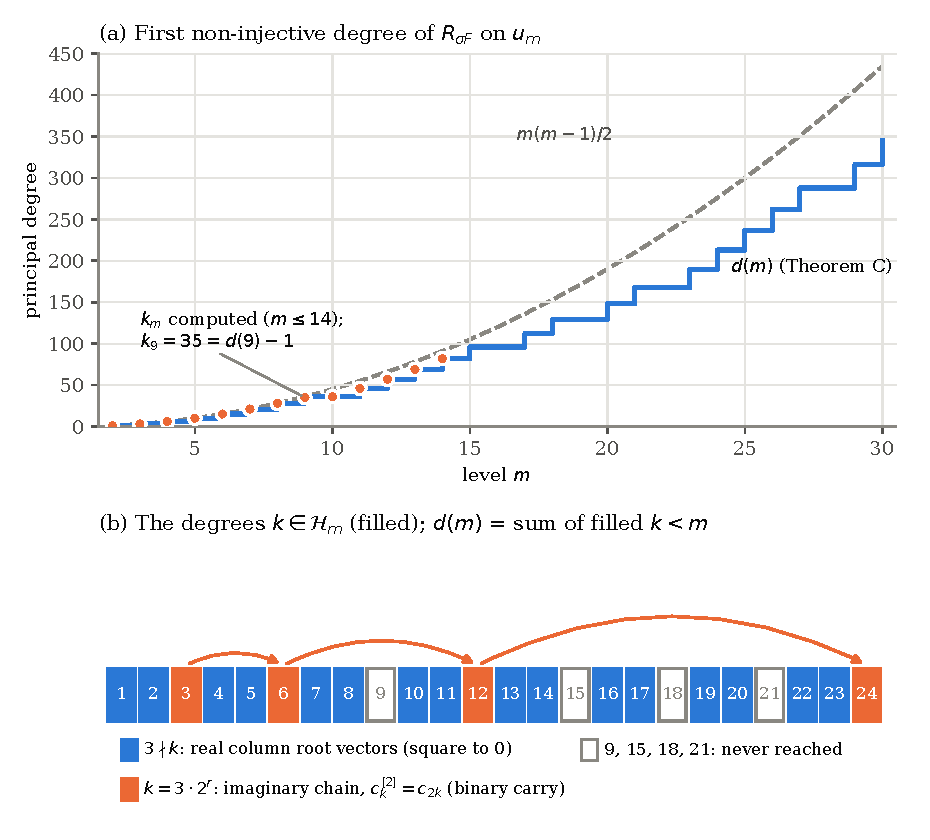
\includegraphics[width=0.92\textwidth]{fig1_threshold_odometer.pdf}
\caption{(a) The first non-injective degree $k_m$ of $R_{\sigma F}$ on $u_m$ (dots, computed for $m\le14$; $k_{15}\le95$)
against $d(m)$ of Theorem~C (steps) and the naive guess $m(m-1)/2$ (dashed). (b) The mechanism: the column subalgebra
generated by $c_1,c_2,c_3$ contains $c_k$ for $3\nmid k$ and the imaginary chain $c_3\to c_6\to c_{12}\to c_{24}$
produced by the $2$-map (a binary carry), but never $c_9,c_{15},c_{18},c_{21},\dots$; the staircase
$\omega=\prod_{k\in\mathcal H_m}c_k$ has degree $d(m)$ and is annihilated by $\sigma F$ (Theorem~\ref{thm:kernel}).}
\label{fig:threshold}
\end{figure}

%======================================================================
\section{The central filtration}\label{sec:filtration}
%======================================================================

\begin{proposition}\label{prop:central}
$L_m$ is central in $L/L_{\ge m+1}$ with zero $2$-map, $u_{m+1}$ is a free module over $\Lambda(L_m)$ with
$u_{m+1}/L_mu_{m+1}=u_m$, and for every degree (and, in the split model, every $Q$-block $\gamma$)
\[
  \dim\ker R^{(m+1)}_\gamma\le\sum_{S}\dim\ker R^{(m)}_{\gamma-\mathrm{wt}(S)},
\]
the sum over subsets $S$ of a homogeneous basis of $L^s_m$. Consequently
\[
  k_{m+1}\ge k_m\qquad\text{and}\qquad \dim\ker R^{(m+1)}/|G_{m+1}|\le\dim\ker R^{(m)}/|G_m| .
\]
\end{proposition}

\begin{proof}
$[L_i,L_m]\subset L_{\ge m+1}$ and $L_m^{[2]}\subset L_{2m}$. With $J=L_mu_{m+1}$, $J^i/J^{i+1}\cong\Lambda^i(L_m)\otimes u_m$
and $R_{\sigma F}$ preserves the $J$-adic filtration with $\gr R=1\otimes R^{(m)}$; apply $\dim\ker f\le\dim\ker\gr f$.
\end{proof}

%======================================================================
\section{$\sigma F$ is a non-zero-divisor}\label{sec:nzd}
%======================================================================

Although $u(L)$ is not a domain (Theorem~\ref{thm:zd}), the leading form of $F$ is regular.

\begin{theorem}\label{thm:nzd}
Left and right multiplication by $\sigma'$ are injective on $U=u(\hatn)=u(L^s)$. Consequently $\sigma F$ is a two-sided
non-zero-divisor in $u(L)=\gr\F_2[[P]]$, $F$ is a two-sided non-zero-divisor in $\F_2[[P]]$, and $k_m\ge m-3$ for all
$m$; in particular $k_m\ge\max(57,m-3)$ for $m\ge12$.
\end{theorem}

\begin{proof}
(1) With $e_i=y_{1,i}$ the three Chevalley generators one checks $\sigma'=e_0e_1e_2+e_1e_2e_0+e_2e_0e_1$.
(2) Let $\rho^*(x)=(\pi(x)+\operatorname{tr}\pi(x)\,I)^{T}$, where $\pi$ is the natural representation of
Proposition~\ref{prop:affine}; this is a graded restricted representation of $L^s$ over $\F_2[t]$, injective on $L^s$,
with $e_0\mapsto tE_{20}$, $e_1\mapsto E_{01}$, $e_2\mapsto E_{12}$, so that $\rho^*(\sigma')=t\cdot I$.
(3) Let $\Psi_r$ be the action of $U$ (via its coproduct) on $V^*(t_1)\otimes\cdots\otimes V^*(t_r)$, with independent
variables $t_i$. Specialising $t_r=0$ makes $\Psi_r(\sigma')$ block upper triangular, and induction gives
$\det\Psi_r(\sigma')|_{(t,0,\dots,0)}=t^{3^r}$; hence $\det\Psi_r(\sigma')\ne0$ and $\Psi_r(\sigma')$ is invertible over
$\F_2(t_1,\dots,t_r)$.
(4) The matrix coefficients of $\rho^*$ generate the graded dual $U^*$ as an algebra: by graded Nakayama it suffices
that they span the indecomposables $Q(U^*)\cong P(U)^*=(L^s)^*$, which holds because $\rho^*$ is injective on $L^s$.
Thus for every $y\ne0$ there is $r$ with $\Psi_r(y)\ne0$, and $\Psi_r(y\sigma')=\Psi_r(y)\Psi_r(\sigma')\ne0$; similarly
on the left. The statement for $\sigma F$ follows by Corollary~\ref{cor:blocks} (injectivity is invariant under
$\otimes\F_8$). Since $\F_2[[P]]$ is complete for the filtration with $\gr\F_2[[P]]=u(L)$, a non-zero-divisor leading
form forces $F$ to be a non-zero-divisor. Finally, $u_m$ and $U$ agree in degrees $<m$, so $R_{\sigma'}$ is injective on $(u_m)_n$ for
$n+3<m$, i.e.\ $k_m\ge m-3$. Each step was also checked by machine; a more detailed write-up of (3) and (4) is in
\texttt{results/THEORY.md}, \S7.1, of the repository.
\end{proof}

\begin{remark}\label{rem:route}
Theorem~\ref{thm:nzd} is the ``Kaplansky part'' of the expected statement $\rk_P(F)=1$; it does not by itself give
$c_e=0$, because $\F_2[[P]]$ is not known to embed in a division ring. The method gives only a linear bound for $k_m$:
on $u_m$ one would need $\Psi_r(\sigma')^{-1}$ to have monomial denominators, but already
$\det\Psi_3(\sigma')=s_1^{21}(s_1^3+t_1t_2t_3)^2$ with $s_1=t_1+t_2+t_3$.
A natural route to a quadratic bound is to show that every kernel element at level $m$ dies at level $m-a$; by
Frobenius duality this is equivalent to $\omega_{K_a}\in u_m\sigma'$, where $\omega_{K_a}$ is the product of all letters
of degree $m-a,\dots,m-1$, and it holds for $a=3$, $6\le m\le10$. However, this route cannot succeed: if
$T_a(m)=\sum_{k=m-a}^{m-1}k\,d_k\le k_{m-a}+2$, then $R_{\sigma'}$ is onto near the top of the ideal generated by $L_{\ge m-a}$
and the integral of $u_{m-a}$ lifts to a kernel element at level $m$, so $\omega_{K_a}\notin u_m\sigma'$. Since
$T_a(m)<3am$ while $k_{m-a}\ge m-a-3$ grows, for every fixed $a$ the criterion fails for infinitely many $m$, and any
chain of such steps yields at most $k_m\le b+4m^{3/2}$, which is just short of what Theorem~\ref{thm:conditional} needs.
A quadratic bound is equivalent to the vanishing of $H_1(L_{\ge m};\,U/U\sigma')$ below degree $c\,m^2$, since
$\ker(R^{(m)})_n\cong\operatorname{Tor}_1^{u(L_{\ge m})}(\F_2,U/U\sigma')_{n+3}$.
\end{remark}

%======================================================================
\section{Computations}\label{sec:numerics}
%======================================================================

\begin{table}[h]
\centering
\begin{tabular}{rrrrrr}
\toprule
$m$ & $|G_m|$ & $\dim C_m$ (exact) & graded cokernel & bound on $c_e$ & $k_m$ \\
\midrule
2 & $2^3$ & 7 & 7 & 0.29167 & 1\\
3 & $2^6$ & 37 & 37 & 0.19271 & 3\\
4 & $2^8$ & 100 & 100 & 0.13021 & 6\\
5 & $2^{11}$ & 547 & 547 & 0.08903 & 10\\
6 & $2^{14}$ & 3170 & 3182 & 0.06449 & 15\\
7 & $2^{16}$ & \textbf{10226} & 10226 & 0.05201 & 21\\
8 & $2^{19}$ & -- & \textbf{64216} & 0.04083 & 28\\
9 & $2^{22}$ & -- & \textbf{423412} & 0.03365 & \textbf{35}\\
10 & $2^{24}$ & -- & \textbf{1526176} & \textbf{0.03032} & 36\\
11 & $2^{27}$ & -- & -- & -- & 46\\
12 & $2^{30}$ & -- & -- & -- & \textbf{57}\\
13 & $2^{32}$ & -- & -- & -- & \textbf{69}\\
14 & $2^{35}$ & -- & -- & -- & \textbf{82}\\
15 & $2^{38}$ & -- & -- & -- & $\le\mathbf{95}$\\
\bottomrule
\end{tabular}
\caption{Exact data. Values for $m\le6$ reproduce \cite[Table~6.1]{ChenIII}; bold entries are new. The bound column
is $\dim C_m/n_m$ for $m\le7$ and (graded cokernel)$/n_m$ for $m\ge8$ (Lemma~\ref{lem:semicont}). $k_m$ is the
first degree where $R_{\sigma F}$ fails to be injective on $u_m$.}
\end{table}

The bounds of the table are plotted in Figure~\ref{fig:bounds}.

\begin{figure}[htbp]
\centering
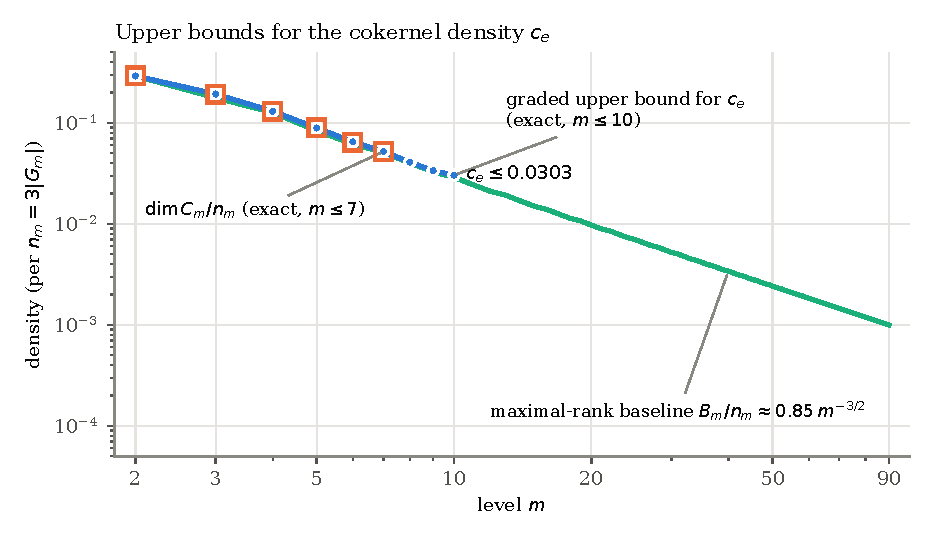
\includegraphics[width=0.92\textwidth]{fig2_ce_bounds.pdf}
\caption{Upper bounds for $c_e$ (log--log). Squares: exact $\dim C_m/n_m$ ($m\le7$). Dots: the graded upper
bound $\dim\coker(R_{\sigma F}|u_m)/n_m$ (Lemma~\ref{lem:semicont}), exact for $m\le10$, giving $c_e\le0.0303$.
Line: the maximal-rank baseline $B_m/n_m$ (Section~\ref{sec:excess}), computed exactly for $m\le90$; the graded
bound equals the baseline plus the excess $e_m/3$, and $c_e=0$ is equivalent (at the graded level) to $e_m\to0$.}
\label{fig:bounds}
\end{figure}

\begin{remark}
The kernel at degree $k_m$ is $3$-dimensional and spanned by $\omega_0,\omega_1,\omega_2$ for $m\in\{2,\dots,8\}\cup\{10,\dots,14\}$.
The case $m=9$ is exceptional: $k_9=35=d(9)-1$, and the kernel there is spanned by the rotations of a ``lowered
staircase'' $\eta$, which is not annihilated by any single letter and arises from a cancellation inside
$\eta\sigma'$; it leaves the kernel at $m=10$. In particular the empirical rule $k_m=m(m-1)/2$, valid for $m\le8$,
fails for $m\ge9$.
\end{remark}

%======================================================================
\section{Maximal-rank baseline and excess}\label{sec:excess}
%======================================================================

Throughout, $h_n=\dim(u_m)_n$, $\mathrm{top}$ is the top degree of $u_m$, $\mathrm{mid}=\mathrm{top}/2$, and
$\ker_n=\dim\ker(R_{\sigma'}|(u_m)_n)$. Let $X_m$ be the degree of a uniformly random PBW monomial of $u_m$, i.e.\
$X_m=\sum_{k<m}\sum_{i=1}^{d_k}k\,\varepsilon_{k,i}$ with independent fair bits $\varepsilon_{k,i}$, so that
$h_n=|G_m|\Pr[X_m=n]$ and $\mathbb E X_m=\mathrm{mid}$.

Trivially $\dim\ker R_\gamma\ge\max(0,\dim u_\gamma-\dim u_{\gamma+\delta})$. Put
$B^Q_m=\sum_\gamma\max(0,\dim u_\gamma-\dim u_{\gamma+\delta})$, and define the excess $e_m$ by
\[
  x_m:=\frac{\dim\ker R_{\sigma F}|u_m}{|G_m|}=\frac{B^Q_m}{|G_m|}+e_m,\qquad c_e\le x_m/3 .
\]

\begin{lemma}\label{lem:anticonc}
There is an absolute constant $A$ with $\max_n\Pr[X_m=n]\le A\,m^{-1/2}$ and
$B_m:=\sum_n\max(0,h_n-h_{n+3})\le A\,m^{-1/2}|G_m|$.
\end{lemma}

\begin{proof}
For each $k<m-3$ with $k\equiv1,2\pmod 6$ pick one letter of degree $k$ and one of degree $k+3$; these $M\ge m/3-2$
pairs are disjoint. Let $T$ be the number of pairs in which exactly one of the two letters occurs. Conditionally on
$T$ and on all other bits, $X_m=Y+3\,\mathrm{Bin}(T,\tfrac12)$ with $Y$ fixed. Hence $\max_n\Pr[X_m=n]$ and the total
variation distance $d_{TV}(X_m,X_m+3)$ are bounded by $\mathbb E[\min(1,A_0T^{-1/2})]$, and $T\sim\mathrm{Bin}(M,\tfrac12)$
gives $O(M^{-1/2})$. Finally $\sum_n(h_n-h_{n+3})=0$, so $B_m=\tfrac12\sum_n|h_n-h_{n+3}|=|G_m|\,d_{TV}(X_m,X_m+3)$.
\end{proof}

Since $B^Q_m$ and $B_m$ agree numerically to four digits, Lemma~\ref{lem:anticonc} shows rigorously that the
degree-wise baseline is $O(m^{-1/2})$; the exact values for $m\le90$ follow $B_m/|G_m|\approx2.55\,m^{-3/2}$, as a local
central limit theorem predicts ($\operatorname{Var}X_m=\tfrac14\sum_{k<m}k^2d_k\sim2m^3/9$).
The excess is small: $e_m=0.0025,\ 0.0022,\ 0.0027,\ 0.0041$ for $m=7,\dots,10$, symmetric about the middle degree.

\begin{conjecture}\label{conj:excess}
$e_m\to0$. Equivalently (given the baseline asymptotics) the graded cokernel density tends to $0$, and hence $c_e=0$.
\end{conjecture}

Conjecture~\ref{conj:excess} is a Lefschetz-type maximal-rank statement for multiplication by the weight-$\delta$
element $\sigma'$ on the truncated restricted enveloping algebras of $\hatn$; compare \cite{Lefschetz} for the
commutative theory. The exceptional element $\eta$ at $m=9$ shows that a proof cannot rest on annihilators alone.

\subsection{The excess is a special-position effect}
The weight-$\delta$ subspace of $u^s_m$ is $6$-dimensional (spanned by $y_{3,0}$, $y_{3,1}$, $y_{2,q}y_{1,q+1}$ and
$y_{1,0}y_{1,1}y_{1,2}$), so all $63$ nonzero $\F_2$-elements can be tested.
\begin{proposition}[proof by computation]\label{prop:generic}
For $4\le m\le 8$, a generic element of $(u^s_m)_\delta$ (over $\overline{\F}_2$) has maximal rank on every $Q$-block,
i.e.\ excess $0$. For $m=9$ its excess is at most $18$, concentrated in $18$ small square blocks near the middle degree.
By contrast $\sigma'$ has excess $3,30,156,162,1136,11200$ for $m=4,\dots,9$.
\end{proposition}
(Maximal rank is certified blockwise by exhibiting one element, over $\F_2$, $\F_{16}$ or $\F_{256}$, of maximal rank;
rank is lower semicontinuous.) Thus the truncated algebras $u^s_m$ have the maximal-rank property for weight $\delta$
almost perfectly, and the excess of $\sigma'$ comes from its special position. Semicontinuity bounds $\rk R_{\sigma'}$
in the wrong direction, so this does not by itself prove Conjecture~\ref{conj:excess}.

\subsection{A conditional proof}

\begin{theorem}\label{thm:conditional}
Suppose that for some constant $C$ and infinitely many $m$:
\begin{enumerate}
\item[(H1)] $\ker_n\le C\,h_{n-k_m}$ for $k_m\le n\le\mathrm{mid}$, and
\item[(H2)] $k_m\ge d(m)-1$.
\end{enumerate}
Then along these $m$
\[
  x_m\le 2C\,\Pr[X_m\le\mathrm{mid}-k_m]+6\max_n\Pr[X_m=n]\le 2C\,e^{-m/4+O(1)}+6A\,m^{-1/2},
\]
and consequently $c_e=0$. In (H2) it suffices that $k_m/m^{3/2}\to\infty$.
\end{theorem}

\begin{proof}
Let $r_n$ be the rank of $R_{\sigma'}:(u_m)_n\to(u_m)_{n+3}$, so $\ker_n=h_n-r_n$. By the duality of
Corollary~\ref{cor:blocks} (summed over blocks of a fixed principal degree), $\ker_n=h_{\mathrm{top}-n}-r_{\mathrm{top}-n-3}$.
Writing $j=\mathrm{top}-n-3$ this reads $\ker_n=(h_{j+3}-h_j)+\ker_j$. Summing over $n>\mathrm{mid}$, the terms
$h_{j+3}-h_j$ telescope to at most $3\max_nh_n$, and the degrees $n$ within $3$ of $\mathrm{mid}$ contribute at most
$3\max_nh_n$ more; hence
\[
  \dim\ker R_{\sigma'}\le 2\sum_{n\le\mathrm{mid}}\ker_n+6\max_nh_n .
\]
By (H1), $\sum_{n\le\mathrm{mid}}\ker_n\le C\sum_{j\le\mathrm{mid}-k_m}h_j=C|G_m|\Pr[X_m\le\mathrm{mid}-k_m]$.
Hoeffding's inequality for $X_m$ (a sum of independent variables with ranges $k$) gives
$\Pr[X_m\le\mathrm{mid}-k_m]\le\exp\bigl(-2k_m^2/\sum_{k<m}k^2d_k\bigr)$; with $k_m\ge d(m)-1\sim m^2/3$ and
$\sum_{k<m}k^2d_k\sim8m^3/9$ the exponent is $-m/4+O(1)$, and it tends to $-\infty$ as soon as $k_m/m^{3/2}\to\infty$.
The last term is bounded by Lemma~\ref{lem:anticonc}. Since $x_m$ is non-increasing (Proposition~\ref{prop:central}),
a subsequence suffices, and $c_e\le x_m/3$.
\end{proof}

Hypothesis (H1) holds with $C=3$ for $5\le m\le10$ (the ratio $\ker_n/h_{n-k_m}$ equals $3$ at $n=k_m$ and decreases
afterwards), and (H2) holds for $m\le 14$: an exact layer-wise lifting from level $10$ gives $k_{12}=57=d(12)$,
$k_{13}=69=d(13)$ and $k_{14}=82=d(14)$ (all $\rho$-orbits of blocks were computed; for $m=14$ the largest block has dimension $16\,769\,439$),
and in each case the kernel at $d(m)$ is exactly the span of $\omega_0,\omega_1,\omega_2$. Hence $R_{\sigma F}$ is injective in all degrees $\le81$ for
every $m\ge14$ (Proposition~\ref{prop:central}). For $m=15$ we found the predicted exceptional element: an element
$\eta_{15}\equiv y_{13,1}\,\omega^{(14)}_0\pmod{L_{14}}$ of degree $95=d(15)-1$ with $\eta_{15}\sigma'=0$, so $k_{15}\le95$; like $\eta$ at $m=9$, it is not annihilated by any single letter and it leaves the kernel at $m=16$.
Injectivity below $95$ was checked only on the smaller blocks of degrees $94$ and $95$ (the only lower bound proved is
$k_{15}\ge k_{14}=82$). For $m=11$ a partial computation (all blocks of dimension $\le 2\cdot10^4$,
remaining blocks bounded via Proposition~\ref{prop:central}) gives $0.00051\le e_{11}\le 0.01693$.

\begin{remark}
The condition $k_m/m^{3/2}\to\infty$ is sharp for this method: if $k_m=O(m^{3/2})$, the central limit theorem keeps
$\Pr[X_m\le\mathrm{mid}-k_m]$ bounded below. One can also show that $k_m\to\infty$ if and only if $R_{\sigma'}$ is
injective on the untruncated algebra $u(\hatn)$, in which case $k_m\ge m-3$; otherwise $k_m$ is eventually constant
($\ge57$). Moreover, the column annihilators of Section~\ref{sec:kernel} cannot by themselves prove (H2): from $m=7$ on,
the dual witnesses for the disappearance of $\omega_j$ at a jump step are of cancellation type.
\end{remark}

%======================================================================
\section{Graded zero divisors do not lift}\label{sec:lift}
%======================================================================

\begin{proposition}[proof by computation]\label{prop:lift}
\begin{enumerate}
\item For every $0\ne v\in V$ and every $x\in\F_2[[P]]$ with leading form $v$, $x^2\in I^9\setminus I^{10}$.
The obstruction is a nonzero class in $\ker\ad_v/\operatorname{im}\ad_v$ in degree $9$.
\item For every pair $(v,w)\in(V\setminus0)^2$ and all lifts $x,y$, $xy\notin I^{11}$.
\item For the $(3,14)$ family of the Remark in Section~\ref{sec:zd}, $xy\in I^{18}\setminus I^{19}$ for all lifts.
\end{enumerate}
\end{proposition}

These statements are exact: they solve the lifting equations as linear systems in $\gr\F_2[[P]]$, enumerating the
full affine solution space where the equations become nonlinear (for instance all $2^9$ choices in (2)). Moreover,
for the lifts $\tilde v$ the kernel density of right multiplication on $\F_2[G_m]$ is $0.375$, $0.279$, $0.234$
for $m=5,6,7$, decreasing like that of a generic element of $I^4$ ($0.332$, $0.244$, $0.203$), whereas in the
graded algebra it stays at $0.625$.
This is consistent with the pro-2 Kaplansky conjecture for $P$, but of course does not prove it.

%======================================================================
\section{Other cyclic algebras}\label{sec:family}
%======================================================================

The construction of Section~\ref{sec:split} makes sense for every prime $p$ and every degree $\ell\ge2$ (we write $\ell$
for the degree, to avoid a clash with $d(m)$ and $d_k$). Let $A^s_{p,\ell}=\F_p^{\ell}[\varphi;s]$ with $s$ the cyclic
shift of the idempotents $e_0,\dots,e_{\ell-1}$, let $t=(1,\dots,1)\varphi^\ell$, and put
$L_{p,\ell}=(A^s_{p,\ell})_{>0}/t\F_p[t]$ with the commutator bracket and the $p$-th power map. Exactly as in
Proposition~\ref{prop:split}, $L_{p,\ell}\otimes\F_{p^\ell}\cong\gr P_{p,\ell}\otimes\F_{p^\ell}$ for the pro-$p$ group
$P_{p,\ell}=(1+\varphi\mathcal O)/(1+t\F_p[[t]])$, $\mathcal O=\F_{p^\ell}[[\varphi;\sigma]]$, $\varphi^\ell=t$, and for
$p\nmid\ell$ the algebra $L_{p,\ell}$ is the positive part of $A_{\ell-1}^{(1)}$ in its principal grading. Write $u_m$,
$k_m$ as before, with $y_{k,i}=e_i\varphi^k$, and let
\[
  \sigma'_{p,\ell}=\sum_{r\in\Z/\ell}e_re_{r+1}\cdots e_{r+\ell-1},\qquad e_i=y_{1,i},
\]
the cyclic sum of the Coxeter word. For $(p,\ell)=(2,3)$ this is the leading form $\sigma'$ of $F$ (step (1) of the proof
of Theorem~\ref{thm:nzd}). We have not constructed lattices and Hecke elements for other $(p,\ell)$; the results of this
section concern the graded model with $\sigma'_{p,\ell}$ as the natural candidate for the leading form. In this
generality the analogue of Theorem~B holds verbatim, the non-zero-divisor theorem extends to all $p\nmid\ell$, and the
explicit kernels of Theorem~C do \emph{not} extend, except for $\ell=2$.
All computations of this section use an independent implementation for general $p$ (Appendix~\ref{app:comp}(f)).

\begin{theorem}\label{thm:famnzd}
If $p\nmid\ell$, then left and right multiplication by $\sigma'_{p,\ell}$ are injective on $u(L_{p,\ell})$; hence
$k_m\ge m-\ell$ for all $m$.
\end{theorem}

\begin{proof}
The proof of Theorem~\ref{thm:nzd} goes through with two changes. First, with
$\pi(e_i)=E_{ii}$, $\pi(\varphi)=\sum_iE_{i+1,i}+tE_{0,\ell-1}$, the map $\rho(x)=\pi(x)-\ell^{-1}\operatorname{tr}\pi(x)\,I$
kills $t\F_p[t]$ and is a restricted representation, because $(X-cI)^p=X^p-c^pI$, $\operatorname{tr}(X^p)=(\operatorname{tr}X)^p$
in characteristic $p$, and $\ell^p\equiv\ell$; this is where $p\nmid\ell$ is used. Second, in
$\rho^*(x)=-\rho(x)^T$ one has $\rho^*(e_i)=-E_{i-1,i}$ for $i\ne0$ and $\rho^*(e_0)=-tE_{\ell-1,0}$, so each cyclic word
maps to $(-1)^\ell tE_{r-1,r-1}$ and $\rho^*(\sigma'_{p,\ell})=(-1)^\ell t\,I$; the triangularity argument then gives
$\det\Psi_r(\sigma'_{p,\ell})|_{(t,0,\dots,0)}=\pm t^{\ell^r}$. Faithfulness is unchanged.
\end{proof}

\begin{remark}
For $p\mid\ell$ the scalar loops are not split off and the argument fails. For $(p,\ell)=(2,2)$ one has
$\sigma'=e_0e_1+e_1e_0=[e_0,e_1]=t=0$, and for $(3,3)$ the Coxeter term $y_{1,0}y_{1,1}y_{1,2}$ of $\sigma'$ has coefficient
$3=0$. Nevertheless $\sigma'$ is injective on $u(L_{p,\ell})$ in all degrees $\le9$ for $(3,3)$ and $\le8$ for $(2,4)$
(exact computation).
\end{remark}

\subsection{The column mechanism is a characteristic-$2$ phenomenon}
Theorem~\ref{thm:kernel} rests on $\sigma'\in c_1u+c_2u+c_3u$ for the column letters $c_k=e_{k-1}\varphi^k$. The same
argument works for any $(p,\ell)$, with $c_1,\dots,c_\ell$, as soon as $\sigma'_{p,\ell}$ lies in
the right ideal $c_1u+\dots+c_\ell u$; the column integrals are then kernel elements in degree
$(p-1)\bigl(\sum_{k<m,\,\ell\nmid k}k+\sum_{\ell p^r<m}\ell p^r\bigr)$.

\begin{proposition}[proof by computation]\label{prop:famcol}
$\sigma'_{p,\ell}$ lies in a column ideal (equivalently, by the rotation symmetry, in all of them) for $(p,\ell)=(2,3)$
and for $\ell=2$, $p=3,5,7$. It lies in no column ideal and in no row ideal (letters $e_j\varphi^k$, $j$ fixed), for
either orientation of the Coxeter word, for
\[
  (p,\ell)\in\{(5,3),(7,3),(3,3),(2,4),(3,4),(2,5),(3,5),(2,7)\}.
\]
For $\ell=2$ the
column ideal contains the whole weight space $u_\delta$. Over $\Z$ (computed modulo a large prime and lifted), the class of
$\sigma'_{\ell}$ modulo the column ideal in weight $\delta$ is $0$ for $\ell=2$, is
$2\,(y_{3,0}-y_{2,0}y_{1,1})$ for $\ell=3$, and has coprime integer coordinates for $\ell=4,5,6$.
\end{proposition}

Thus for $\ell=3$ the explicit kernels of Theorem~\ref{thm:kernel} exist only because of the factor $2$ in this class,
and for $\ell\ge4$ they do not exist for any $p>\ell$ nor for the small $p$ tested. In the cases without the column
mechanism the first kernel lies elsewhere: for $(5,3)$ one finds $k_3=14>12$.

\subsection{The case $\ell=2$, $p$ odd}
Put $x_k=y_{k,0}$, $f_k=y_{k,1}$ ($k$ odd) and $h_k=y_{k,0}$ ($k$ even). Then
$[x_i,f_j]=2h_{i+j}$, $[h_j,x_i]=x_{i+j}$, $[h_j,f_i]=-f_{i+j}$, all other brackets of letters vanish,
$x_k^{[p]}=f_k^{[p]}=0$, $h_j^{[p]}=h_{pj}$, and $\sigma'=x_1f_1+f_1x_1=2x_1f_1-2h_2$: the loop algebra of
$\mathfrak{sl}_2$ in its principal grading, and $\sigma'$ is the anticommutator of the two Chevalley generators.

\begin{theorem}\label{thm:famtwo}
Let $p$ be odd, $\ell=2$, $m\ge3$.
\begin{enumerate}
\item $H=\operatorname{span}\{x_k:k\ \text{odd}\}\oplus\operatorname{span}\{h_{2p^r}\}$ is a restricted subalgebra with
$\sigma'\in Hu$, so its integral $\omega_H$ lies in $\ker R_{\sigma'}$, in degree
$\mathrm{od}_p(m)=(p-1)\bigl(\sum_{k<m\ \mathrm{odd}}k+\sum_{2p^r<m}2p^r\bigr)$.
\item $K=\operatorname{span}\{x_k\ (k\equiv1),\ f_k\ (k\equiv3),\ h_k\ (k\equiv0)\bmod 4\}$, the image of the loop algebra under
$t\mapsto t^2$, is a restricted subalgebra, and for $0\le j<p$
\[
  f_1^j\,\sigma'\equiv-2(2j+1)\,h_2f_1^j\pmod{Ku_m}.
\]
Hence $\omega_Kf_1^j\in\ker R_{\sigma'}$ if and only if $j=(p-1)/2$, in degree
\[
  \kappa_p(m)=(p-1)\sum_{k<m,\ k\not\equiv2\ (4)}k+\frac{p-1}2 .
\]
\end{enumerate}
Consequently $k_m\le\min(\mathrm{od}_p(m),\kappa_p(m))$.
\end{theorem}

\begin{proof}
For a restricted subalgebra $K$ let $\omega_K$ be the product of the $(p-1)$-st powers of a homogeneous basis; as in
Lemma~\ref{lem:integral} it spans the right integrals of $u(K)$, so $\omega_Kk=0$ for $k\in K$. Hence $zv\in Ku_m$
implies $\omega_Kzv=0$. By PBW $u_m=u(K)\otimes V$ and $u_m/Ku_m\cong V$ has the PBW monomials in the letters outside $K$ as a basis. (1) Both terms
of $2x_1f_1-2h_2$ begin with a letter of $H$. (2) Closure of $K$: $[x_{4a+1},f_{4b+3}]=2h_{4(a+b+1)}$,
$[h_{4a},x_{4b+1}]=x_{4(a+b)+1}$, $[h_{4a},f_{4b+3}]=-f_{4(a+b)+3}$, $h_{4a}^{[p]}=h_{4ap}$. Since $f_3\in K$ commutes with
$f_1$ and $[h_2,f_1]=-f_3$, one has $f_1^ah_2f_1^b\equiv f_1^{a+b}h_2\equiv h_2f_1^{a+b}$ modulo $Ku_m$. Expanding
$[x_1,f_1^j]=2\sum_{a+b=j-1}f_1^ah_2f_1^b$ gives $f_1^jx_1f_1\equiv-2j\,h_2f_1^j$ and $f_1^{j+1}x_1\equiv-2(j+1)\,h_2f_1^j$,
because $x_1(\cdots)\in Ku_m$. The sum is $-2(2j+1)h_2f_1^j$, and $h_2f_1^j$ is a basis vector of $V$.
\end{proof}

Both families were also checked by direct multiplication in $u_m$ ($p=3$: $m\le16$; $p=5$: $m\le12$; $p=7$: $m\le10$),
including the uniqueness of the exponent $(p-1)/2$. At $p=2$ the coefficient $-2(2j+1)$ vanishes identically, in
accordance with $\sigma'_{2,2}=0$. Asymptotically $\mathrm{od}_p(m)\sim(p-1)m^2/4<\kappa_p(m)\sim3(p-1)m^2/8$, so the second
family matters only for small $m$.

\begin{table}[h]
\centering
\begin{tabular}{rrrrrrrrrrrr}
\toprule
$p$ & $m$ & 2 & 3 & 4 & 5 & 6 & 7 & 8 & 9 & 10 & 11\\
\midrule
3 & $\min(\mathrm{od},\kappa)$ & 2 & 3 & 9 & 12 & 22 & 27 & 41 & 48 & 66 & 66\\
3 & $k_m$ & 2 & 3 & 9 & 12 & 22 & 27 & 41 & 48 & \textbf{64} & 66\\
5 & $\min(\mathrm{od},\kappa)$ & 4 & 6 & 18 & 24 & 44 & 44 & & & & \\
5 & $k_m$ & 4 & 6 & 18 & 24 & \textbf{42} & 44 & & & & \\
7 & $\min(\mathrm{od},\kappa)$ & 6 & 9 & 27 & 36 & 66 & & & & & \\
7 & $k_m$ & 6 & 9 & \textbf{26} & \textbf{34} & $\ge63$ & & & & & \\
\bottomrule
\end{tabular}
\caption{Thresholds for $\ell=2$ (exact). Bold: levels where $k_m$ is below the bound of Theorem~\ref{thm:famtwo}.}
\label{tab:famtwo}
\end{table}

At every level of Table~\ref{tab:famtwo} without a bold entry, the kernel in degree $k_m$ is spanned by the elements of
Theorem~\ref{thm:famtwo} and their images under the symmetry $x\leftrightarrow f$. The bold entries are explained by
cancellation-type elements of the kind met at $m=9,15$ in Section~\ref{sec:excess}: at $p=3$, $m=10$ the kernel in degree
$64$ is spanned by a $24$-term lowering of $\omega_H$ and its mirror image. In every case the defect is at most $2$ and the
element dies at the next level. For $p=3$, $m=11$ this gives $k_{11}=66$ by the following window argument. If $n<k_a+a$,
the reduction $u_m\to u_a$ is injective on $\ker(R_{\sigma'}|(u_m)_n)$, block by block: filter $u_m$ by the powers of the
right ideal generated by $L_{\ge a}/L_{\ge m}$ as in the proof of Proposition~\ref{prop:central}; a kernel element in the
$i$-th step, $i\ge1$, would have a leading part in $\gr^iu(L_{\ge a})\otimes\ker R^{(a)}$ of $u_a$-degree $\le n-a<k_a$. With
$a=10$, $k_{10}=64$ it suffices to check the six blocks that carry the level-$10$ kernel in degrees $64$ and $65$; all six
have zero kernel at level $11$, and $\omega_H$ gives $k_{11}\le66$.

The density behaves differently from the case $(2,3)$. Splitting $x_m=\dim\ker R_{\sigma'}/\dim u_m$ into the degree
baseline $\sum_n\max(0,h_n-h_{n+2})/\dim u_m$ and an excess (this only overestimates the excess $e_m$ of
Section~\ref{sec:excess}, which uses the block baseline $B^Q_m$), one finds:
\begin{center}
\begin{tabular}{lll}
\toprule
case & levels & excess\\
\midrule
$\ell=2$, $p=3$ & $m=4,\dots,9$ & $0.0082,\ 0.0082,\ 0.0021,\ 0.00081,\ 0.00012,\ 0.00006$\\
$\ell=2$, $p=5$ & $m=4,5,6$ & $0.0026,\ 0.0015,\ 0.00033$\\
$(2,3)$, $e_m$ & $m=7,\dots,10$ & $0.0025,\ 0.0022,\ 0.0027,\ 0.0041$\\
\bottomrule
\end{tabular}
\end{center}
The baseline is $O(m^{-1/2})$ by Lemma~\ref{lem:anticonc}, whose proof works with shift $2$. So the graded analogue of
$c_e$ vanishes for $\ell=2$ if and only if the excess tends to $0$, and the data support this much more strongly than
for $(2,3)$. Theorem~\ref{thm:conditional} transfers verbatim with $\deg\sigma'=2$: (H1) together with
$k_m\ge\min(\mathrm{od}_p(m),\kappa_p(m))-O(1)$, or merely $k_m/m^{3/2}\to\infty$, implies that the graded cokernel
density tends to $0$.

%======================================================================
\section{Questions}
%======================================================================

\begin{question}
Prove Conjecture~\ref{conj:excess}, or directly that $\rk_P(F)=1$. By Theorem~\ref{thm:conditional} it suffices to prove
(H1) and (H2): the kernel of $R_{\sigma'}$ below the middle degree grows no faster than a fixed multiple of the
free module generated in degree $k_m$, and the threshold stays within one of $d(m)$.
\end{question}

\begin{question}
Is $k_m\in\{d(m)-1,d(m)\}$ for all $m$? More precisely, is it true that $k_m=d(m)-1$ if $3\mid m$, $m\ge9$ and
$m\ne3\cdot2^r$, and otherwise $k_m=d(m)$ with kernel spanned by $\omega_0,\omega_1,\omega_2$? This was formulated from
the data for $m\le12$ and then confirmed for $m=13,14$ ($k_{13}=69$, $k_{14}=82$); for $m=15$ the predicted exceptional
kernel element in degree $95$ exists.
\end{question}

\begin{question}
Show that $\operatorname{Tor}_1^{u(L_{\ge m})}(\F_2,\,u(\hatn)/u(\hatn)\sigma')$ vanishes in degrees below $c\,m^2$ for
some $c>0$ (or below $m^{3/2}\psi(m)$ with $\psi\to\infty$). This is equivalent to the threshold bound needed in (H2), and
by Remark~\ref{rem:route} it cannot be obtained by iterating level-by-level comparisons.
\end{question}

\begin{question}
Is there a filtration of $\F_2[[P]]$ (for instance a weight filtration adapted to the twisted form of $\hatn$) whose
associated graded ring is a domain? By Proposition~\ref{prop:hilbert} such a ring would have subexponential growth,
hence be Ore; if moreover $\F_2[[P]]$ then embeds continuously into a division ring $Q$ with a discrete valuation,
\cite[Thm.~7.1]{JZS} ($\varphi^\#\rk_Q\le\rk_P$) would give $\rk_P(x)=1$ for all $x\ne0$, in particular $c_e=0$.
\end{question}

\begin{question}
(a) Is $\sigma'_{p,\ell}$ a non-zero-divisor when $p\mid\ell$ (Remark after Theorem~\ref{thm:famnzd})?
(b) For $\ell=2$, $p$ odd: is $k_m\ge\min(\mathrm{od}_p(m),\kappa_p(m))-2$ for all $m$, and does the excess tend to $0$?
Here $\mathfrak{sl}_2$-representation theory might replace the evaluation-module arguments of Section~\ref{sec:nzd}.
(c) For $\ell\ge3$, $(p,\ell)\ne(2,3)$: which mechanism produces the first kernel of $R_{\sigma'_{p,\ell}}$?
(d) Lattices acting simply transitively on the vertices of $\tilde A_{\ell-1}$-buildings are obtained from cyclic division
algebras over $\F_q(t)$ \cite{LSV}. Is the leading form of the corresponding Hecke element (the analogue of $F$, now
$1-\bar f\cdots\bar f$ since the Laplacian is $-I+A$ modulo $p$) the cyclic Coxeter sum $\sigma'_{p,\ell}$?
\end{question}

%======================================================================
\appendix
\section{Computational methods}\label{app:comp}
%======================================================================

All code, data and logs are in the repository cited on the title page (directories \texttt{code/},
\texttt{data/} and \texttt{results/}); the figures are produced by the script
\texttt{make\_data\_and\_figures.py}. The group $G_m$ is realised as normalised
truncated skew power series in $\F_8[[\varphi;\sigma]]/(\varphi^m)$, with conventions ported line by line from
Chen's published scripts \cite{ChenIII}. Ranks over $\F_2$ use a bit-packed elimination with $64$-column panels
and Four-Russians tables (numba). Independent checks:
(a) $\dim C_m$ for $m\le6$ reproduces \cite{ChenIII};
(b) $\dim C_7$ was computed from three matrices of provably equal rank (transpose, left multiplication, random
row and column permutations);
(c) $u(L)$ was implemented twice (the $\F_8$-model and the split model, with independent straightening codes) and
checked against Jennings products in $\F_2[G_N]$ for $N\le12$;
(d) the zero divisor of Theorem~\ref{thm:zd} was confirmed by plain group multiplication in $\F_2[G_9]$;
(e) the graded cokernels for $m=9,10$ use the block decomposition of Corollary~\ref{cor:blocks}; for $m=10$ one block
per rotation orbit was computed and the remaining blocks were spot-checked;
(f) Section~\ref{sec:family} uses a second, independent engine for general $p$ and $\ell$ (directory
\texttt{code/family/}): monomials with exponents $<p$ encoded in base $p$, a compiled rewriting system with coefficients,
and rank computations modulo $p$. A pure-Python version and a compiled version agree with each other on $21$ test cases
and reproduce the $(2,3)$ values of Table~1 for $m\le7$ (kernel dimensions and thresholds).

\subsection*{Acknowledgements}
Computations and parts of the analysis were carried out with the assistance of an AI system (Claude, Anthropic).

\begin{thebibliography}{99}
\bibitem{ChenIII} R.~Chen, \emph{Algorithmic Non-commutative Class Field Theory, Volume III: Higher-Rank Buildings,
Non-Equilibrium Topology and Higher-Order Games}, 2026, doi:10.5281/zenodo.23109523.
\bibitem{CMSZ} D.~I.~Cartwright, A.~M.~Mantero, T.~Steger, A.~Zappa, Groups acting simply transitively on the vertices
of a building of type $\tilde A_2$, I, \emph{Geom.\ Dedicata} 47 (1993), 143--166; II: The cases $q=2$ and $q=3$,
\emph{ibid.}, 167--223.
\bibitem{JZsurvey} A.~Jaikin-Zapirain, $L^2$-Betti numbers and their analogues in positive characteristic, in:
\emph{Groups St Andrews 2017 in Birmingham}, LMS Lecture Note Ser.\ 455, Cambridge Univ.\ Press, 2019, 346--406.
\bibitem{JZS} A.~Jaikin-Zapirain, H.~Souza, Sylvester domains and pro-$p$ groups, \emph{Doc.\ Math.} 31 (2026), no.~2, 453--502, doi:10.4171/DM/1034 (theorem numbers as in arXiv:2402.14130v2).
\bibitem{Jennings} S.~A.~Jennings, The structure of the group ring of a $p$-group over a modular field,
\emph{Trans.\ Amer.\ Math.\ Soc.} 50 (1941).
\bibitem{Quillen} D.~Quillen, On the associated graded ring of a group ring, \emph{J.\ Algebra} 10 (1968).
\bibitem{LarsonSweedler} R.~G.~Larson, M.~E.~Sweedler, An associative orthogonal bilinear form for Hopf algebras,
\emph{Amer.\ J.\ Math.} 91 (1969).
\bibitem{Kac} V.~G.~Kac, \emph{Infinite dimensional Lie algebras}, 3rd ed., Cambridge Univ.\ Press, 1990.
\bibitem{Lefschetz} T.~Harima, T.~Maeno, H.~Morita, Y.~Numata, A.~Wachi, J.~Watanabe, \emph{The Lefschetz Properties},
Lecture Notes in Math.\ 2080, Springer, 2013.
\bibitem{LSV} A.~Lubotzky, B.~Samuels, U.~Vishne, Explicit constructions of Ramanujan complexes of type $\tilde A_d$,
\emph{European J.\ Combin.} 26 (2005), 965--993.
\bibitem{EL} M.~Ershov, W.~L\"uck, The first $L^2$-Betti number and approximation in arbitrary characteristic,
arXiv:1206.0474.
\bibitem{Fraczyk} M.~Fraczyk, Growth of mod-2 homology in higher rank locally symmetric spaces, arXiv:1801.09283.
\end{thebibliography}

\end{document}
